
\begin{figure*}[h] % two pictures
	\centering
	\begin{subfigure}[t]{0.48\linewidth}
%		\caption{{\bfseries DNN model 1} \\* Полносвязная однослойная модель}
		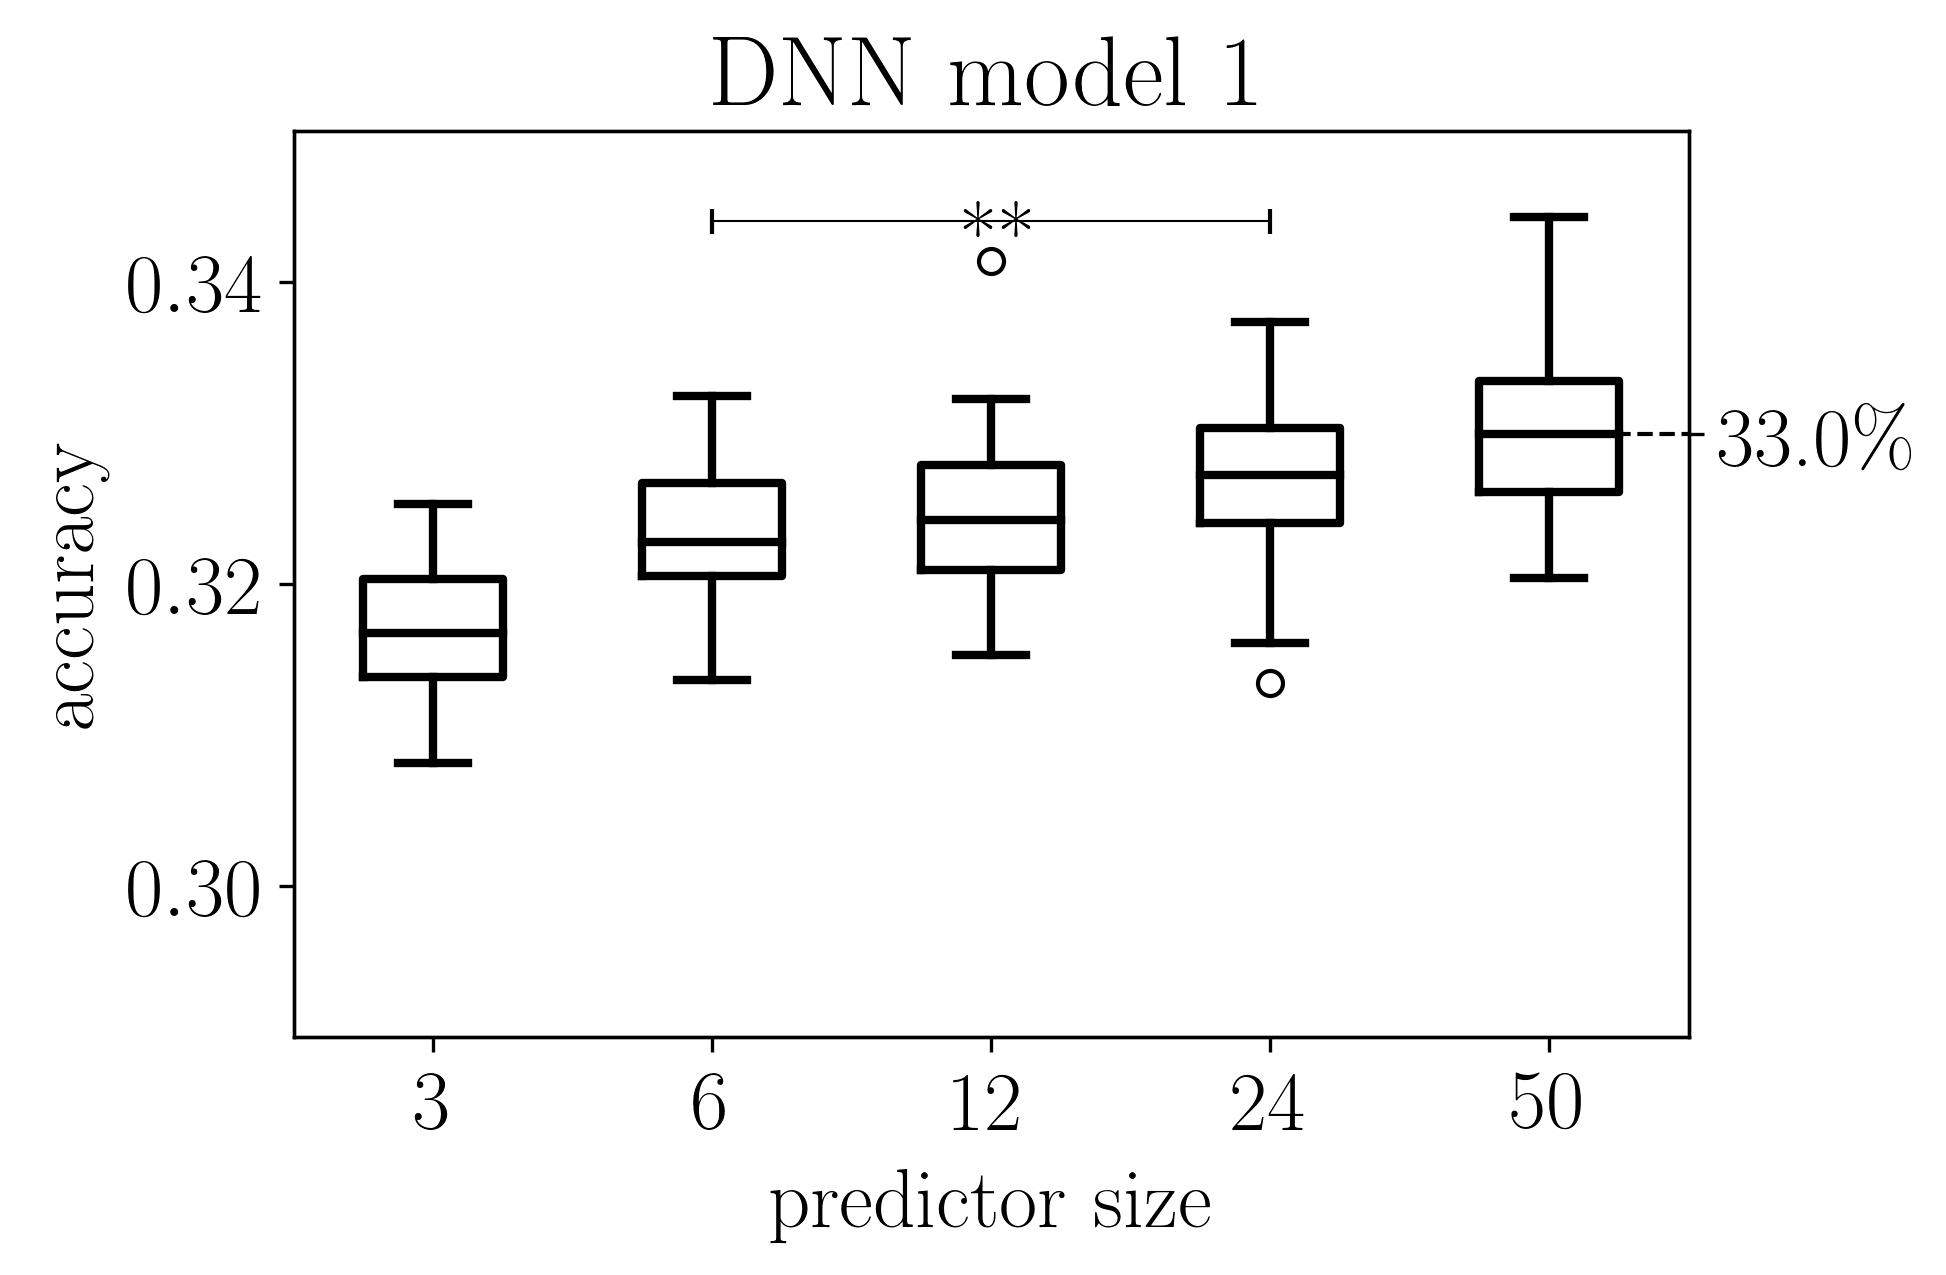
\includegraphics[width = \textwidth]{pics/dnn_model_1_all_runs_p1_ecoli_100000_10000_all_0.png}
		\label{fig:alpha}
	\end{subfigure}
	\begin{subfigure}[t]{0.48\linewidth}
%		\caption{mm}
		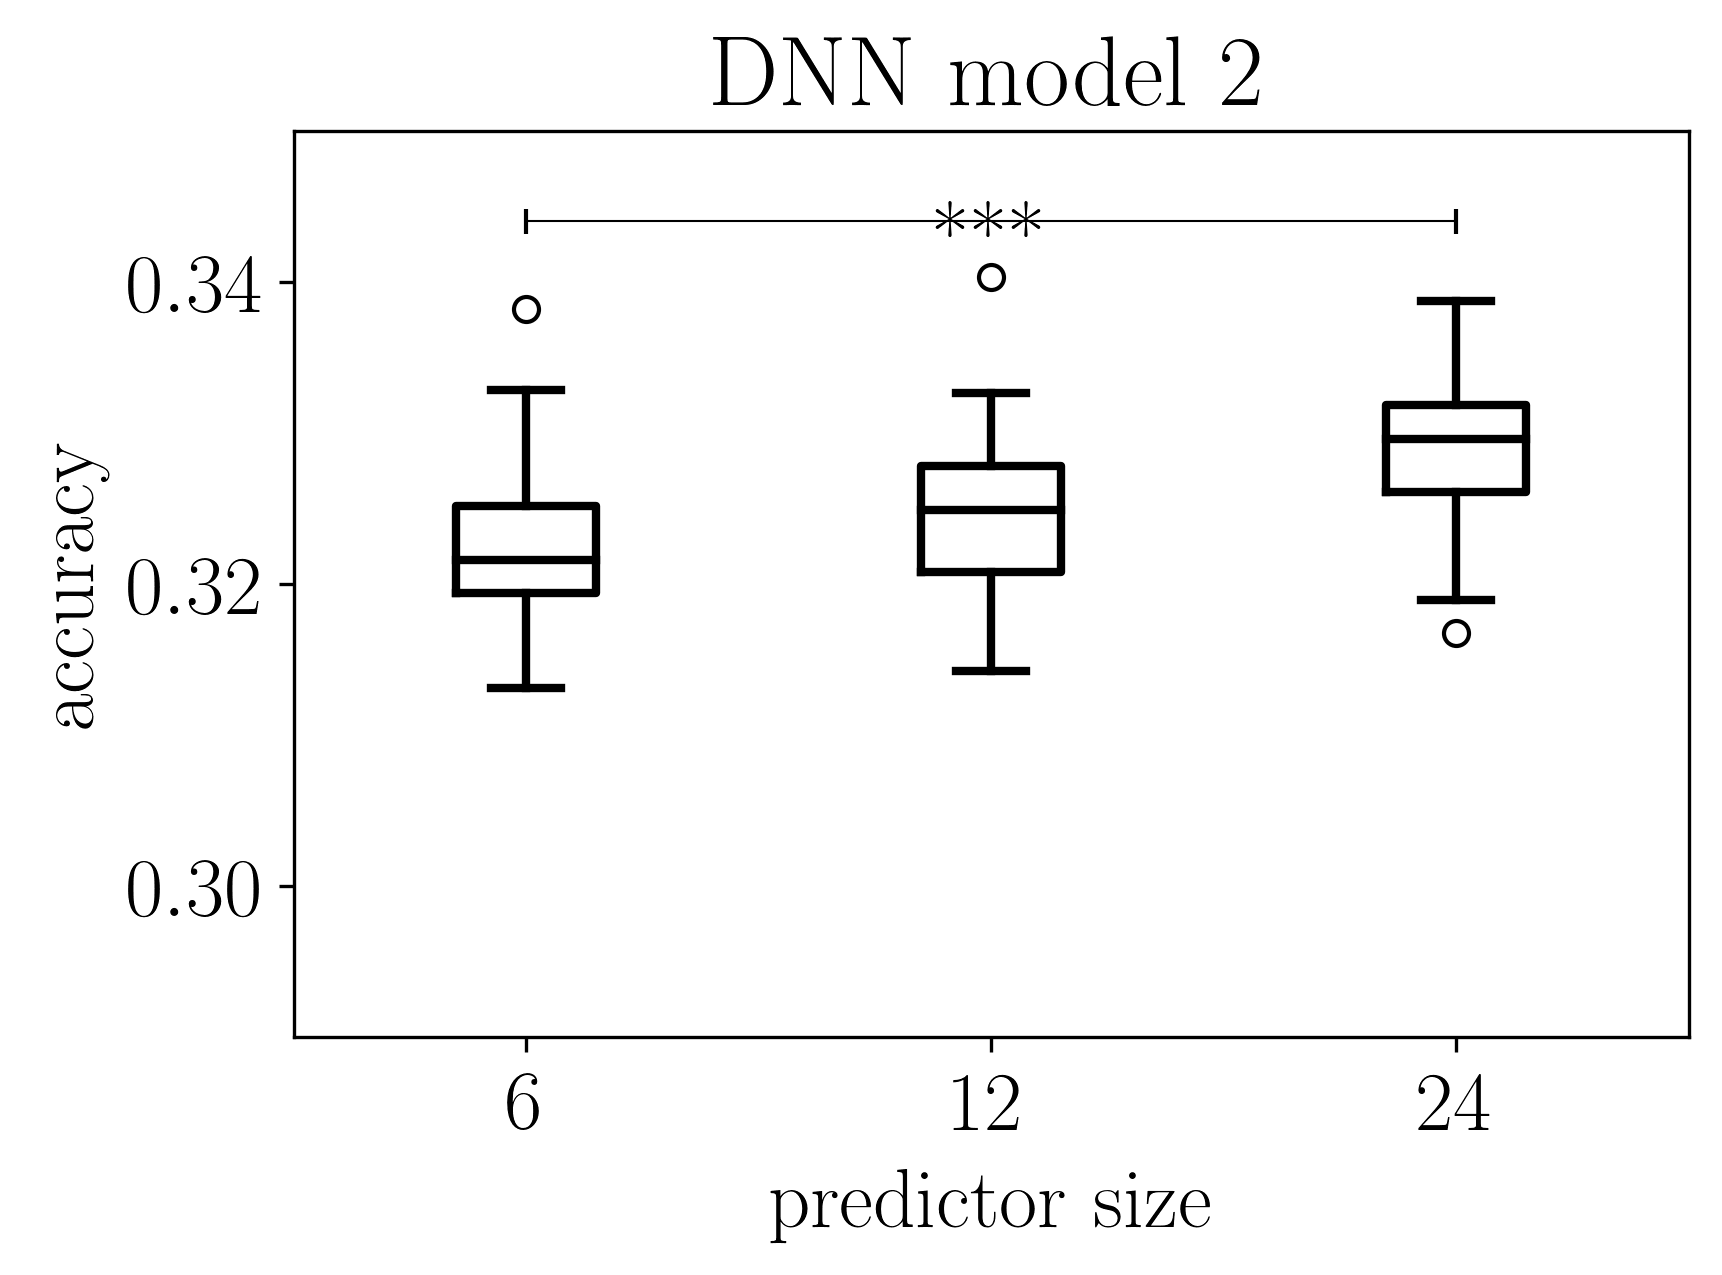
\includegraphics[width = \textwidth]{pics/dnn_model_2_all_runs_p1_ecoli_100000_10000_all_0.png}
			\label{fig:alpha}
	\end{subfigure}
	\begin{subfigure}[]{0.48\linewidth}
%		\caption{{\bfseries CNN model 1} \\* Сверточная однослойная модель }
		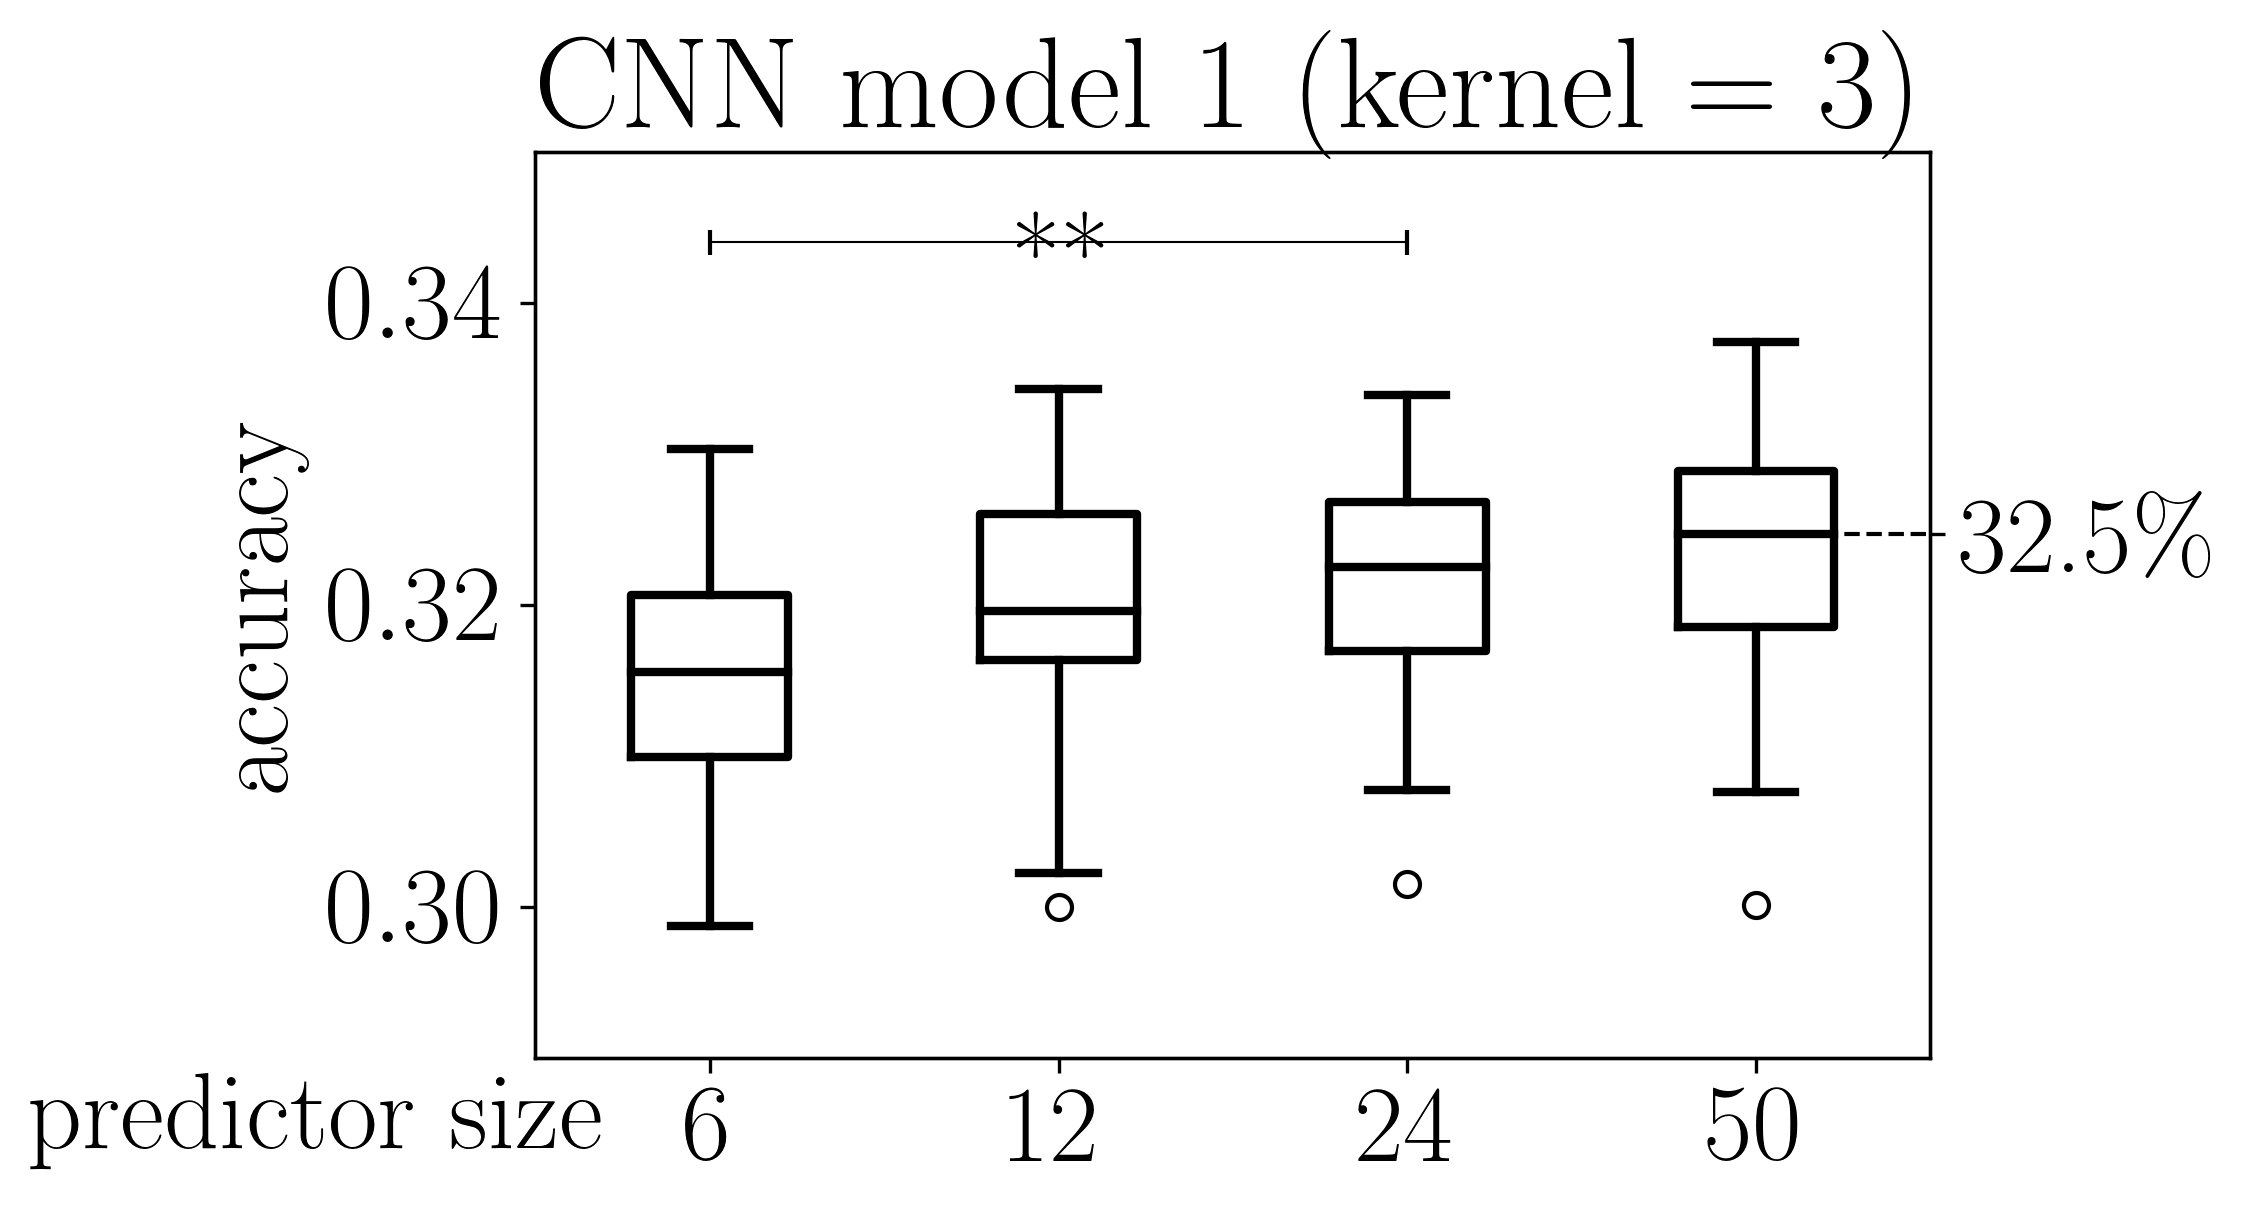
\includegraphics[width = \textwidth]{pics/cnn_model_1_all_runs_p1_ecoli_100000_10000_all_0.png}
		\label{fig:beta}
	\end{subfigure}
	\begin{subfigure}[]{0.48\linewidth}
%		\caption{{\bfseries CNN model 1} \\* Сверточная однослойная модель }
		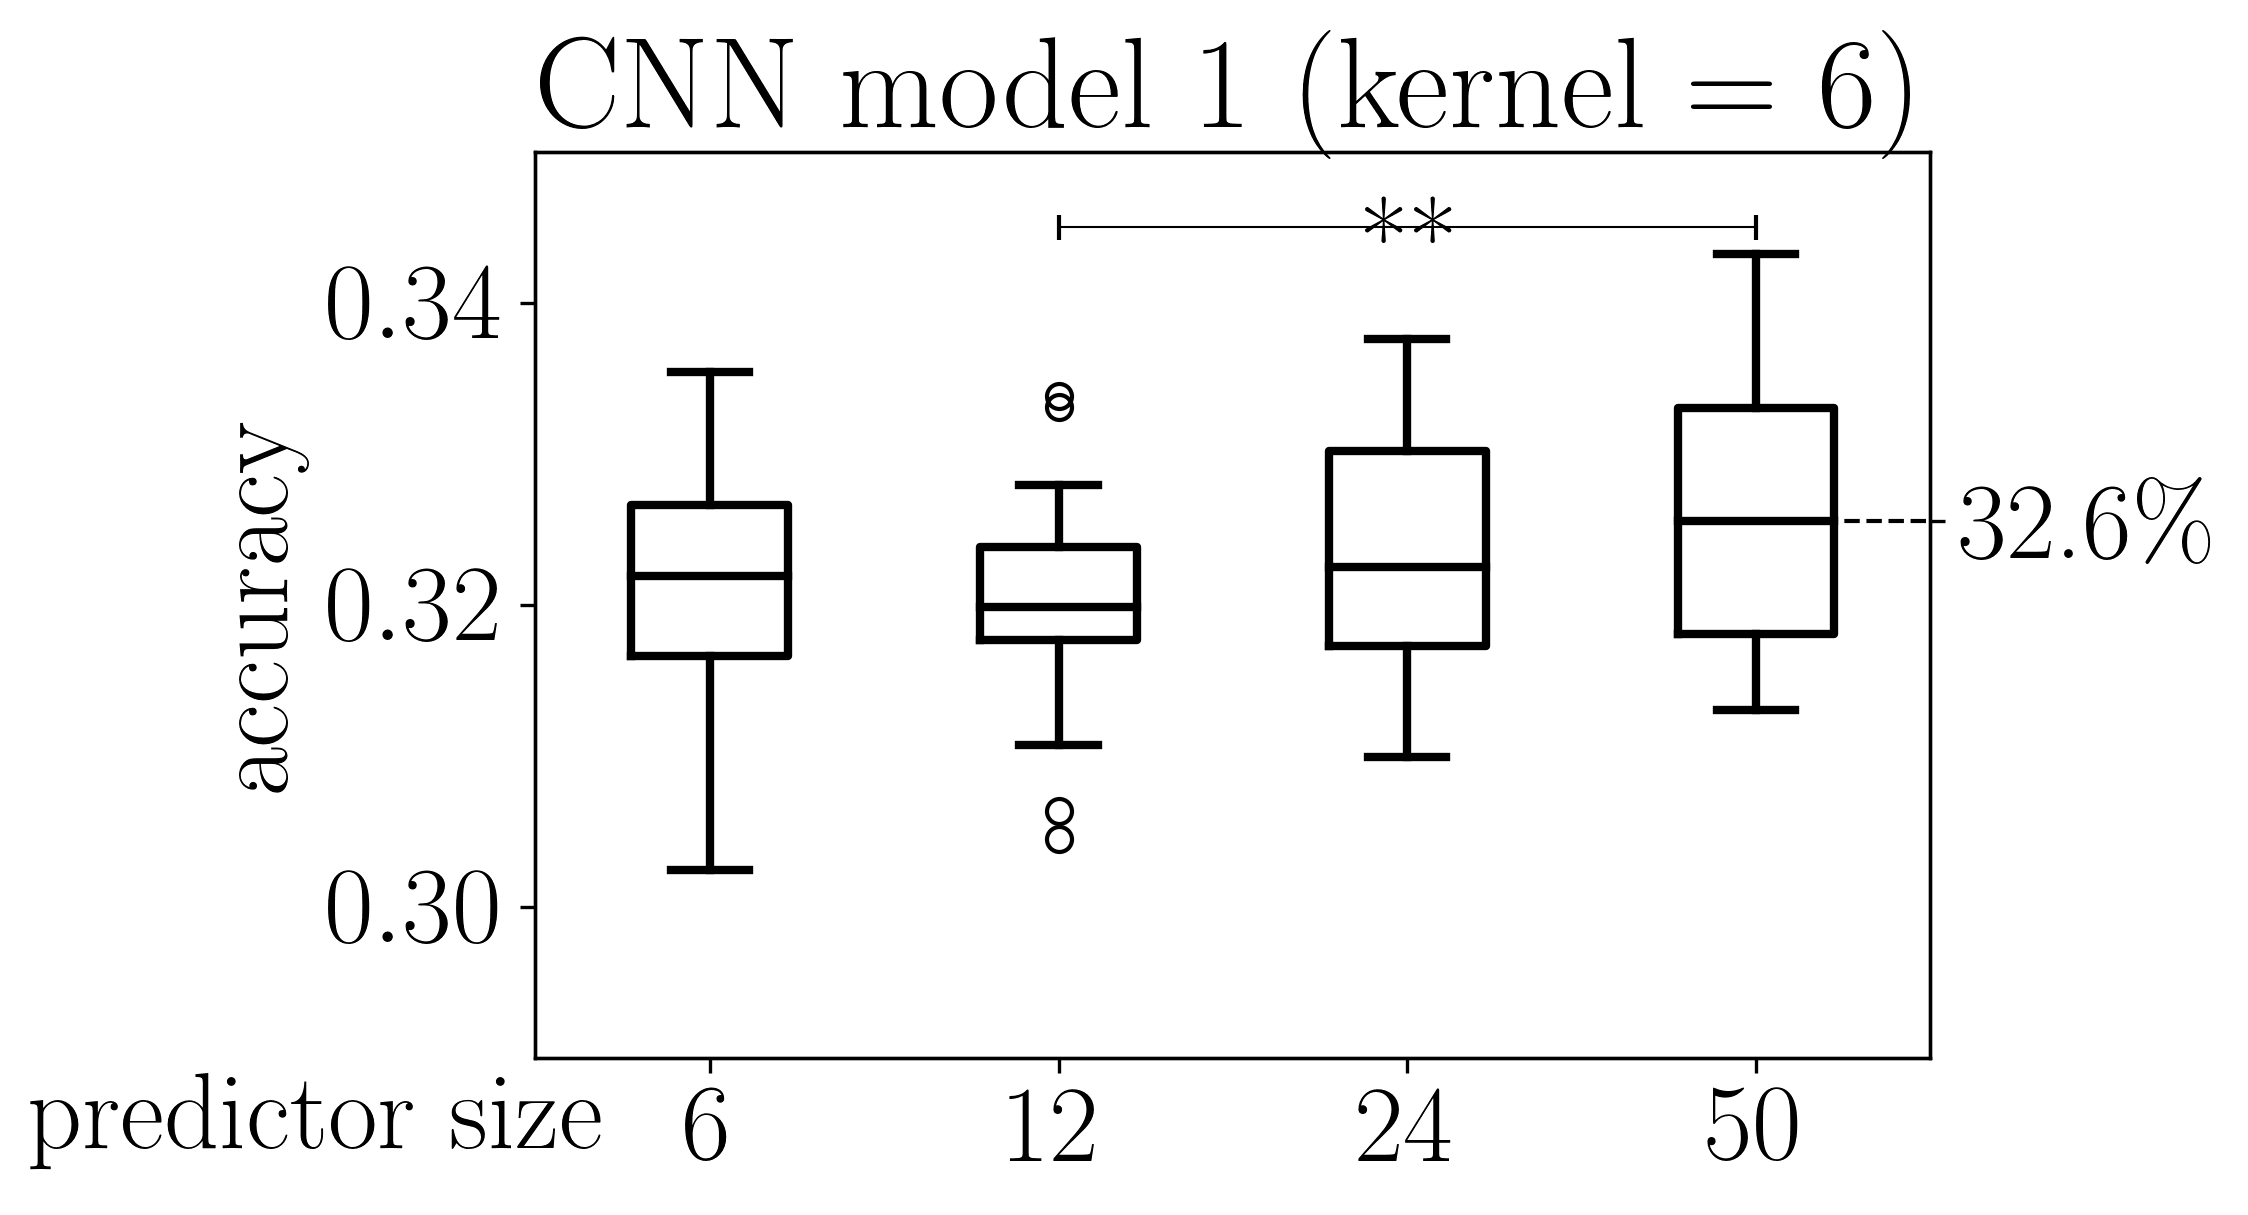
\includegraphics[width = \textwidth]{pics/cnn_model_2_all_runs_p1_ecoli_100000_10000_all_0.png}
		\label{fig:cnn_2_predictor}
	\end{subfigure}
	\caption{{\bfseries Зависимость точности предсказания от размера предикторной области для различных архитектур.} \\*
	По горизонтальной оси обозначен размер области. По вертикальной оси показано распределение точностей обученной модели в сете из 30 запусков с различными наборами данных.}
	
	\label{fig:size}
	
\end{figure*}